\subsubsection{Channel and Buffer Model Paradigms}
\label{ssec:channel}

\begin{figure}
\begin{center}
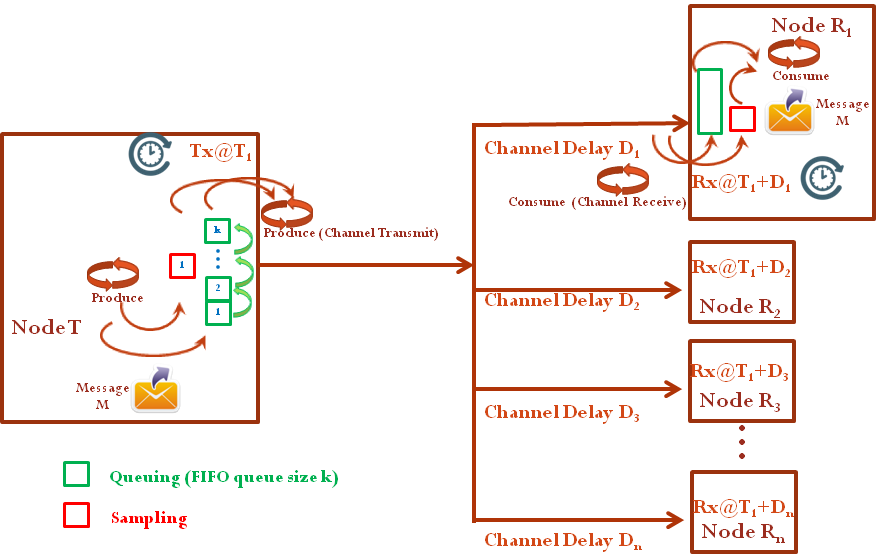
\includegraphics[width=0.8\textwidth]{figures/channel_buffer.png}
\caption{Channel and Buffer Models}
\label{fig:channel_buffer}
\end{center}
\end{figure}

System designers typically have to contend with managing resource constraints across networked systems. There are two high level resources they need to balance: (i) platform resources like CPU utilization (time) and memory (space) vs (ii) network resources like bandwidth/link usage manifesting as transport/channel delay (time) and network card memory/channel buffers (space). Since both platform and network resources along both time and space dimensions are all finite, optimizing along just one of those resources and/or dimension at the cost of the other is not a viable option.  Hence in safety critical avionics domain, both platform and network resources are explicitly time and space partitioned (statically and apriori configured) to ensure adequate allocation of resources thereby guaranteeing correct operation of the system very time. 

Thus Correct characterization of computation time, communication time (channels delay) and associated buffers (memory at platform or network) at every node is a critical element of the ADSL as it lays the foundation for accurate modeling of platform and network resources in the system.  We show the time and space attributes of network resources in terms of channel and buffer models in Figure~\ref{fig:channel_buffer}. We do not show the platform time and space resources (like computation time, memory etc) but it is straightforward extension to the models we have specified there from the perspective of a channel (network). 

For the purpose of our study, channel is modeled as \emph{unidirectional} flow of message $M$ from a transmitter Node $T$ to multiple receiver Nodes $R_1,R_2,...,R_n$ with corresponding channel delays $D_1,D_2,...,D_n$. Channel delays are all different because there may be different transport paths from transmitter to the different receivers. Channel delays are a function of the size of message $M$, the network bandwidth/link rates, the propagation time (wire length) and the number of intermediate relays between transmitter and the receiver. Thus a message transmitted on to the channel at time $T_1$ from Node $T$ is received at each of the receiver from the channel at times $T_1+D_1, T_1+D_2, T_1+D_3,...,T_1+D_n$ respectively.

Also note that as shown in the Figure~\ref{fig:channel_buffer}, there is string of \emph{producing} processes and \emph{consuming} processes in the model and this must correctly identified in-order and in-sequence to get the modeling of the buffer (e.g. overflow or size) correct and this is described next. For example, in Node $T$, there is some platform application that is producing a message (possibly from a computation process) and this produced message is stored in the channel buffer (network card memory). The network card in Node $T$ subsequently reads from its own memory (channel buffer) and produces (transmits) the message on to the channel. 

The process is then reversed at the receiver. The receiver network card consumes the message from the channel and stores the message locally into own channel buffer (network card memory). Then either the network card reads from its channel buffer and pushes the message to consuming platform process OR the consuming platform process reads from the channel buffer and then finally processes the message as it sees fit (possibly sent to a computation process).

Once the processes are correctly modeled as stated above, then we identify two types of channel buffers at either the transmitter or at the receivers:
\begin{itemize}
\item \emph{Queuing}: First-in-First-Out (FIFO) Order i.e. messages are taken out of the queue in the order in which data was produced into it.  The maximum size of the queue is also specified upfront $k$. If messages are not consumed at fast enough rate compared to rate at which message are produced into the buffer and once the queue is already filled with   “k” messages yet to be consumed, then produced message(s) are dropped. Not supported in year I and year II, but in year III

\item \emph{Sampling}: New message produced overwrites old message if not consumed. Supported in year I and year II

\end{itemize}
